\documentclass[aspectratio=169]{beamer}
\usepackage{tikz}
\usepackage{amsmath}
\usepackage{algorithm}
\usepackage{algorithmic}
\usepackage{xcolor}

\definecolor{usccardinal}{rgb}{0.6, 0.0, 0.0}
\definecolor{tropicalrainforest}{rgb}{0.0, 0.46, 0.37}

\usetikzlibrary{shapes,arrows,positioning,calc}
\usetheme{metropolis}
\setbeamercolor{background canvas}{bg=white}

\title{Semi-supervised Continuous Function Learning for Unstructured Data}
\date{CS 846, Fall 2016}
\author{Vineet John}

\begin{document}
\maketitle


\section{Motivation}

\begin{frame}{Motivation}

	\begin{columns}[T] % align columns
		\begin{column}{.45\textwidth}
			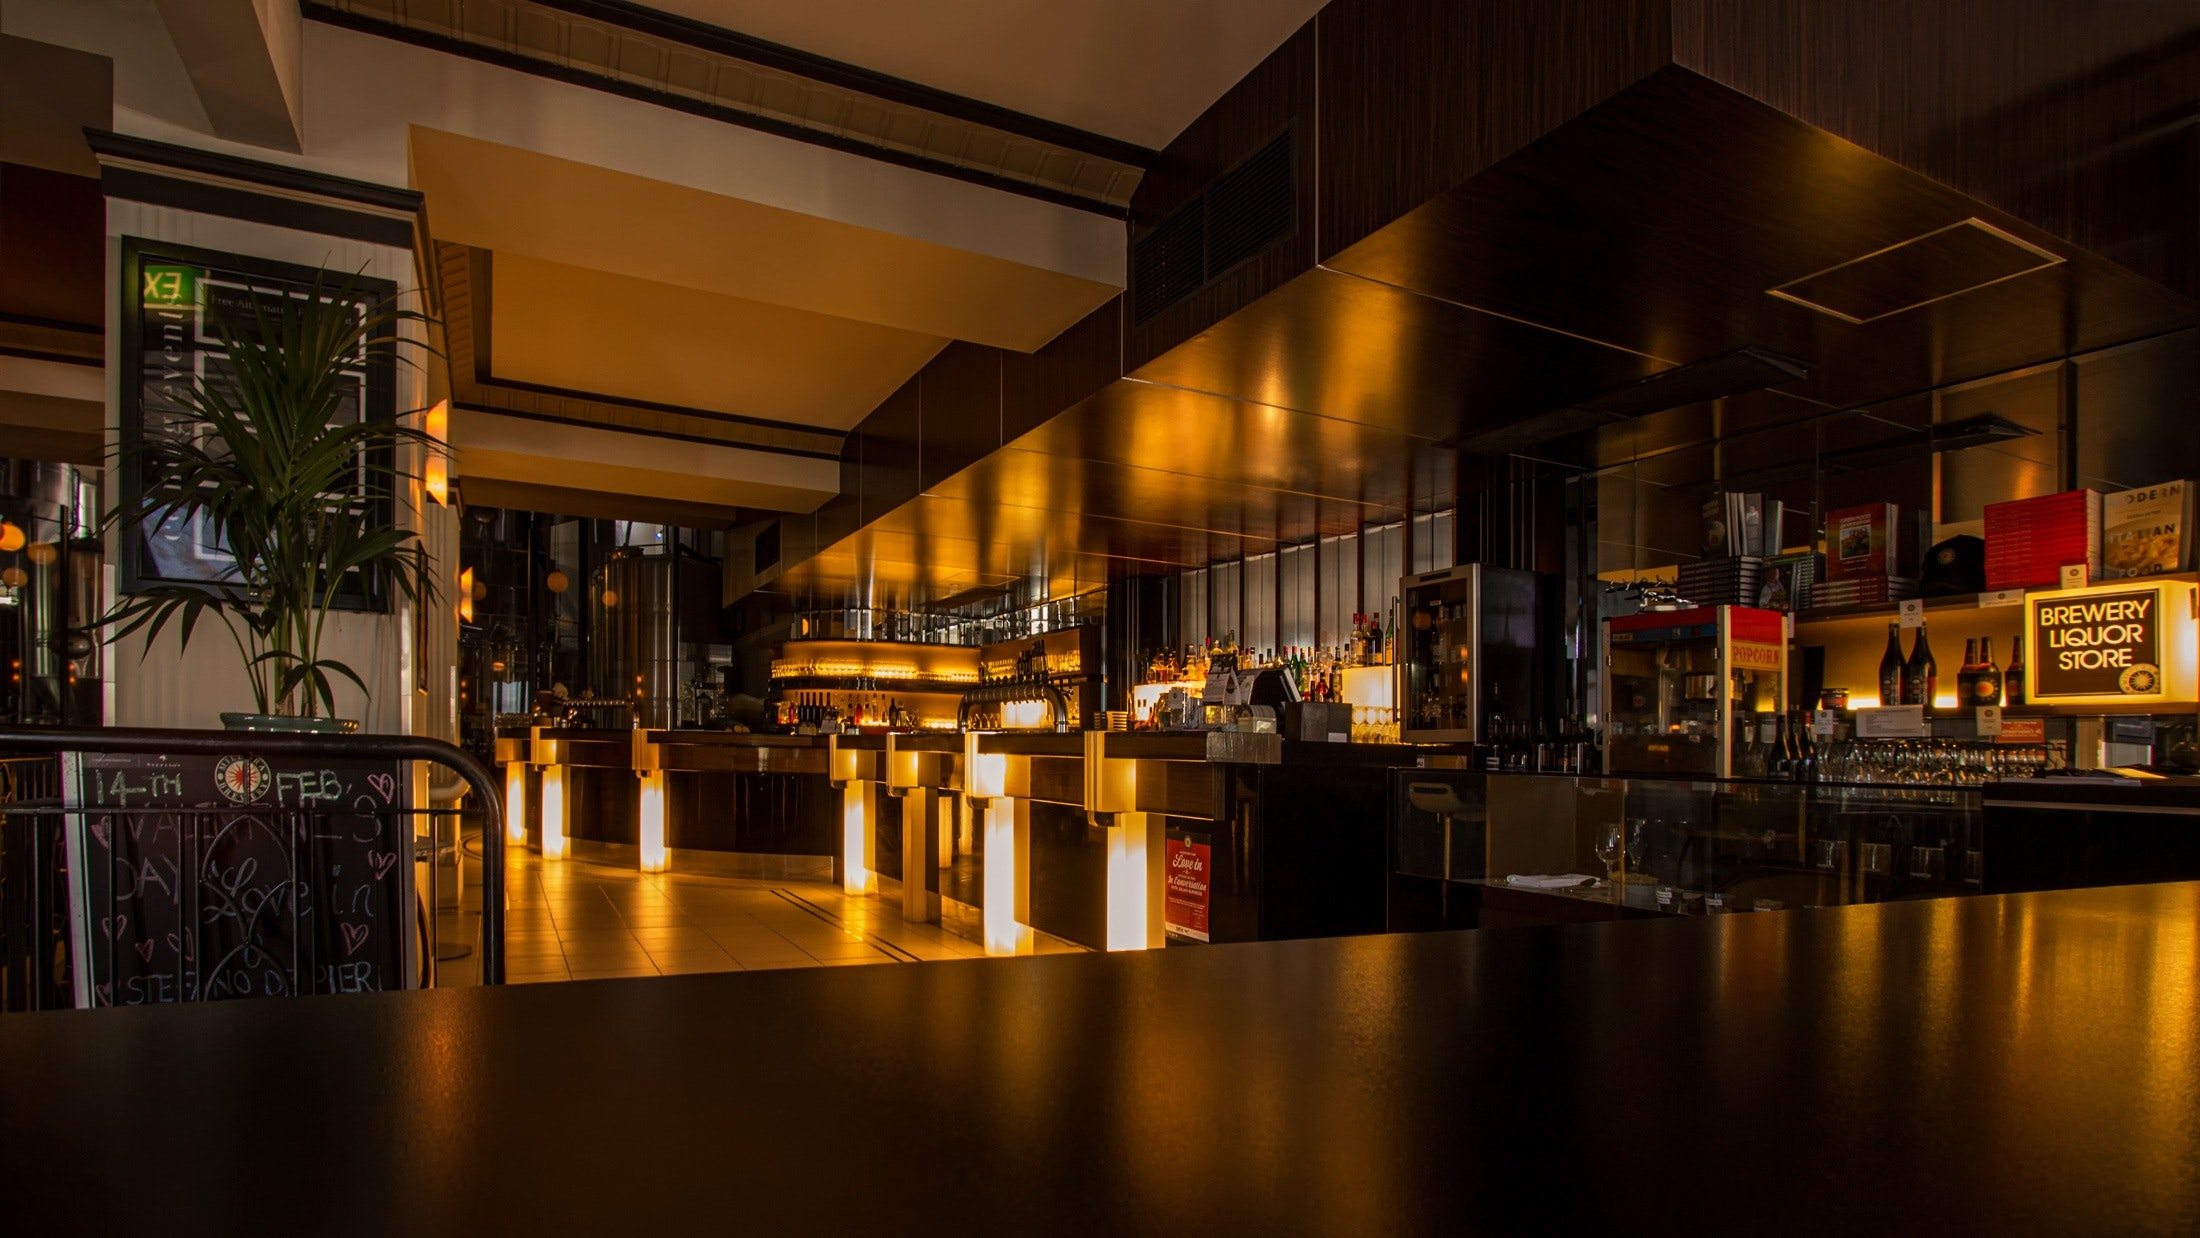
\includegraphics[width=.9\textwidth]{images/restaurant.jpg}
		\end{column}
		\hfill
		\begin{column}{.45\textwidth}
			\textbf{Sources of structured customer feedback}:
			\begin{itemize}
				\item Yelp
				\item TripAdvisor
				\item Amazon
				\item Google Maps
			\end{itemize}
		\end{column}
	\end{columns}
\end{frame}

\begin{frame}{Motivation}

	\begin{columns}[T] % align columns
		\begin{column}{.45\textwidth}
			
\includegraphics[width=.9\textwidth]{images/twitter-status.png}
		\end{column}
		\hfill
		\begin{column}{.45\textwidth}
			\textbf{Sources of {\color{red}unstructured} customer feedback}:
			\begin{itemize}
				\item Twitter
				\item Facebook
				\item Bulletin Board Forums
			\end{itemize}
		\end{column}
	\end{columns}
\end{frame}

\begin{frame}{Motivation}
	\centering
	{\Huge Challenges} \\
	\vspace{1cm}
	\begin{center}
		\begin{minipage}{0.4\textwidth}
			\begin{itemize}
				\item Discrete, High-dimensional
				\item Slang, dialects
				\item Sarcasm, irony
			\end{itemize}
		\end{minipage}
	\end{center}
\end{frame}

\begin{frame}{Motivation}
	\centering
	{\Huge Problem Statement} \\
	\vspace{1cm}
	{\Large Build a semi-supervised framework that leverages \textbf{labeled data sources} to build a \textbf{online query service} for unstructured data from the \textbf{same distribution}}
\end{frame}

\section{Background}

\begin{frame}{Word Embeddings}
	\centering
	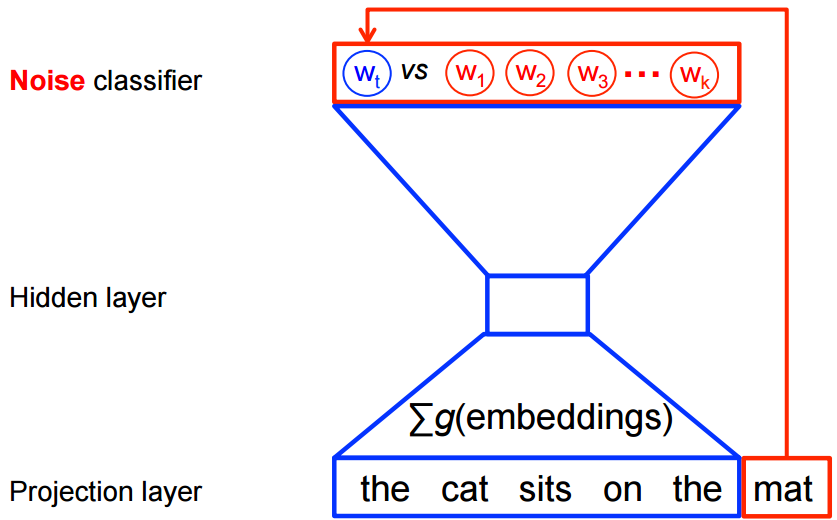
\includegraphics[width=.7\textwidth]{images/word2vec-1.png}
\end{frame}

\begin{frame}{Word Embeddings}
	\centering
	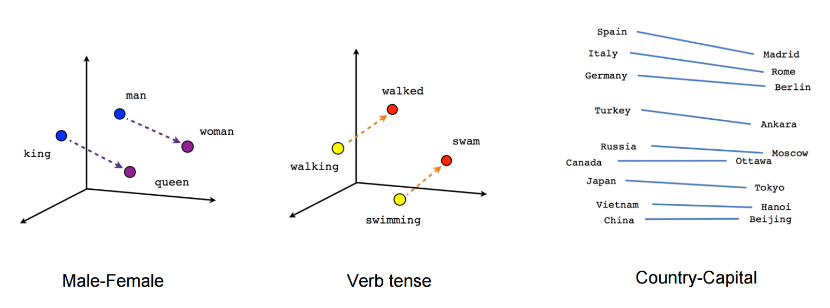
\includegraphics[width=.9\textwidth]{images/word2vec-2.png}
\end{frame}

\begin{frame}{Document Embeddings}
	\centering
	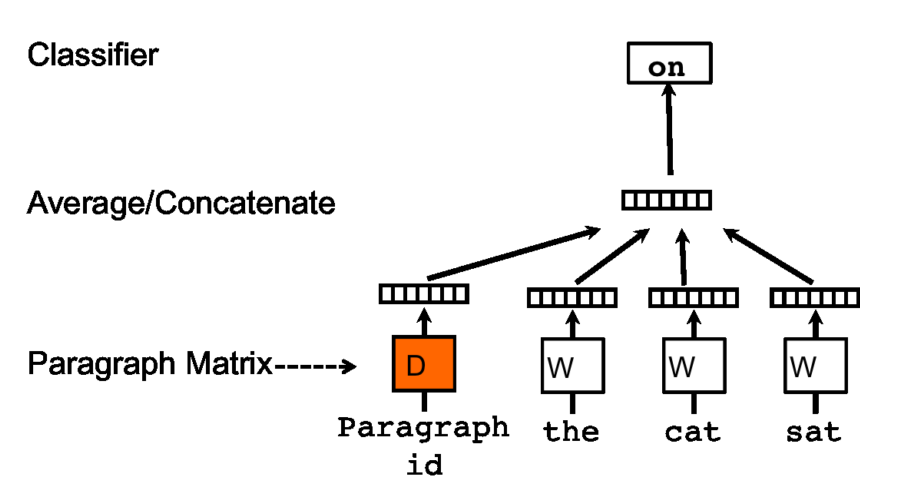
\includegraphics[width=.7\textwidth]{images/docvec.png}
\end{frame}


\section{Implementation}

\begin{frame}{Packages Used \& Data Sources}
	\begin{columns}[T] % align columns
		\begin{column}{.3\textwidth}
			{\Large Libraries}
			\begin{itemize}
				\item NLTK, spaCy
				\item Gensim
				\item Scikit-Learn
			\end{itemize}
		\end{column}
		\hfill
		\begin{column}{.6\textwidth}
			{\Large Data}
			\begin{itemize}
				\item Amazon Book Reviews
				\item 8.9GB, approximately 8.9 million reviews
				\item 60K randomly selected training reviews, 1K validation, 10K test
			\end{itemize}
		\end{column}
	\end{columns}
\end{frame}

\begin{frame}{Architecture}
	\centering
	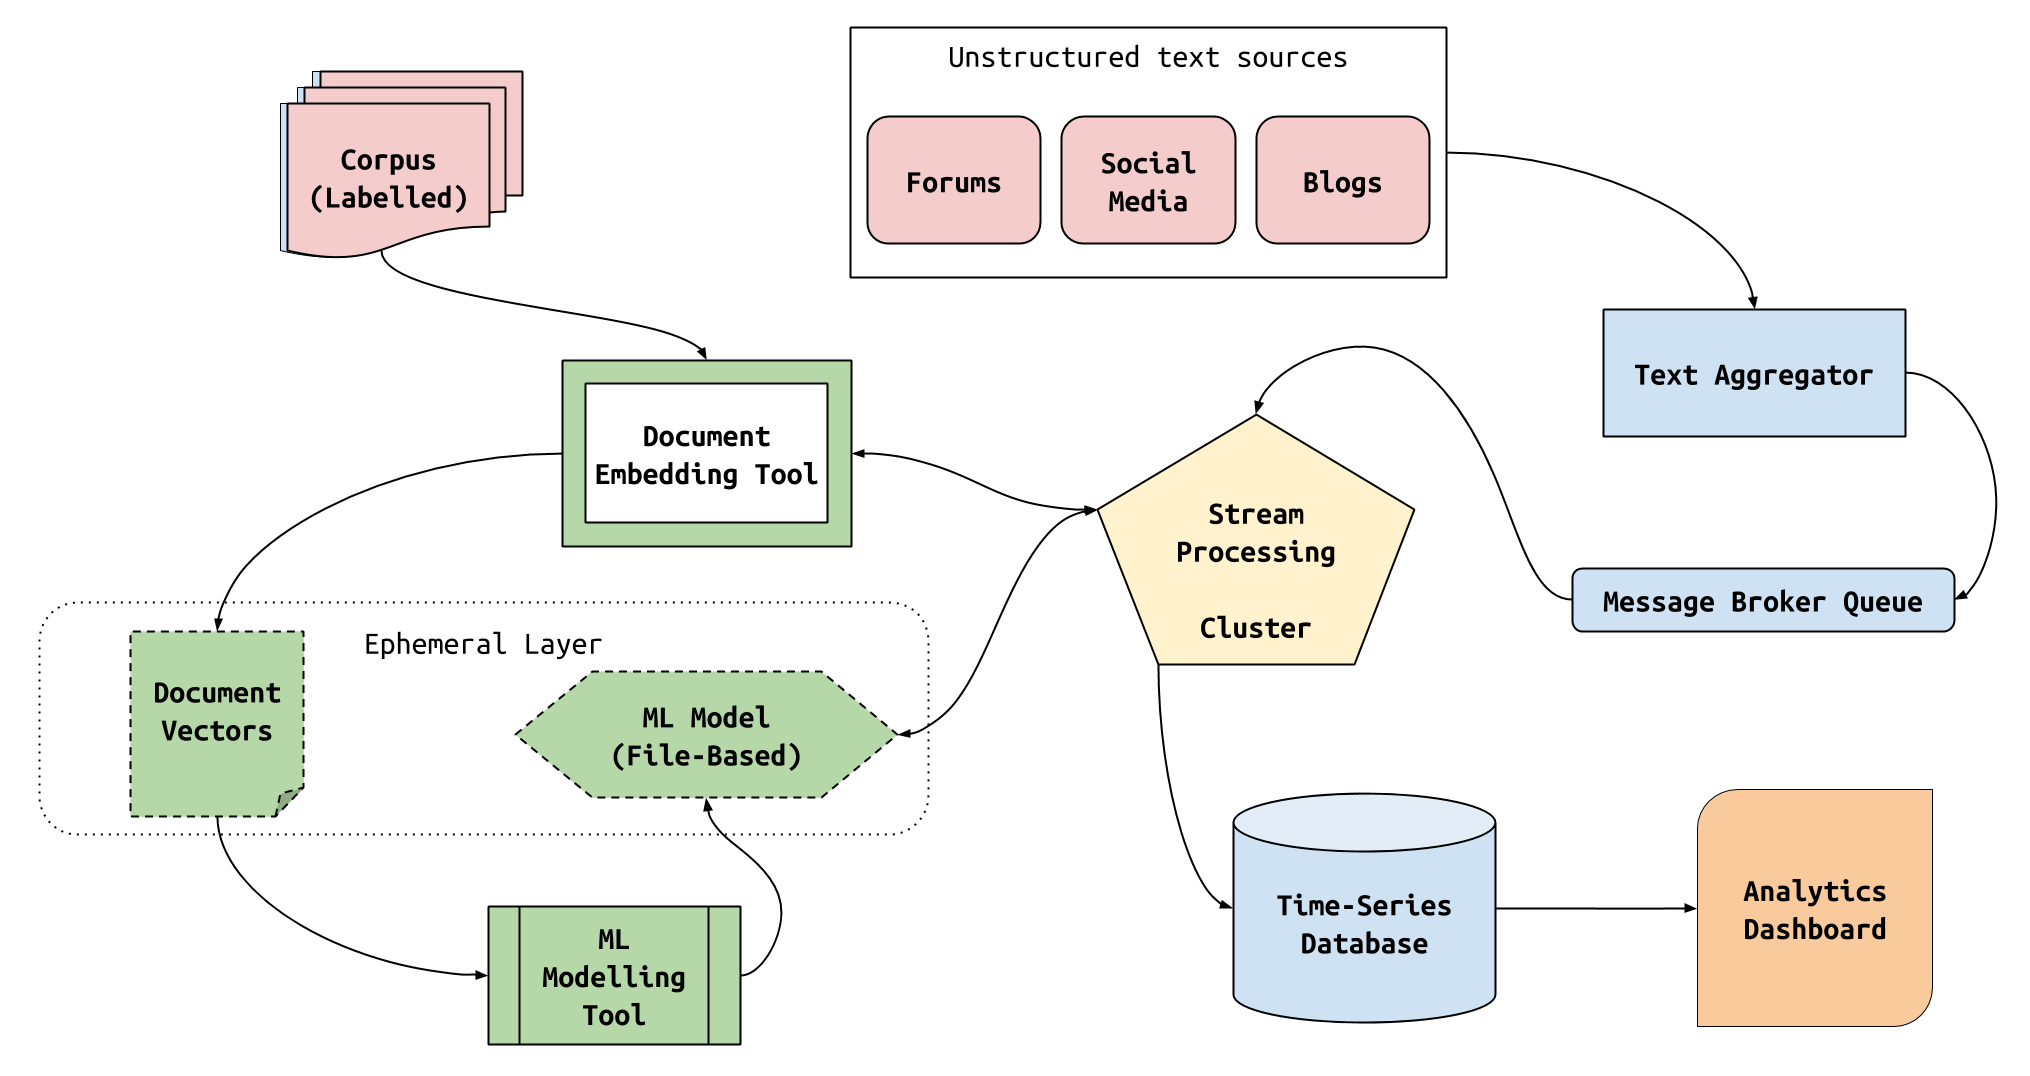
\includegraphics[width=.9\textwidth]{images/rapid-rate-system-arch.png}
\end{frame}


\section{Results}

\begin{frame}{Results}
	\centering
	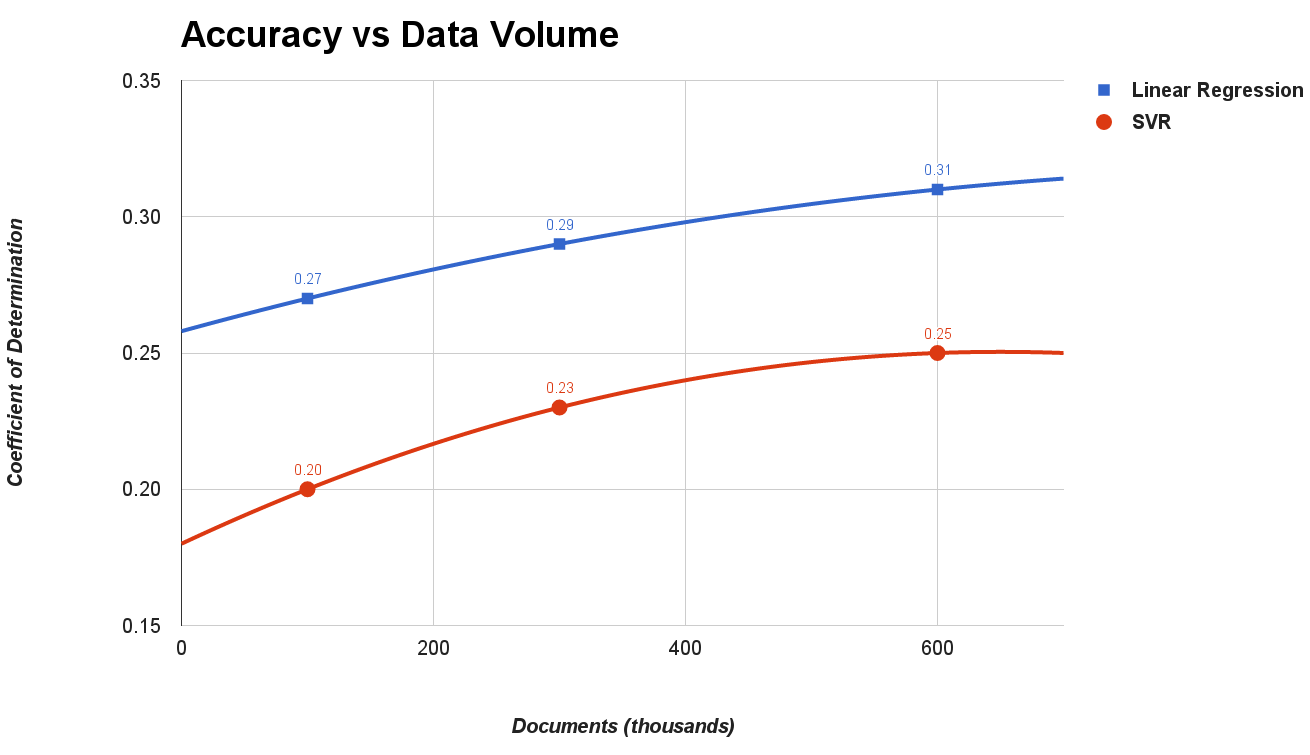
\includegraphics[width=.9\textwidth]{images/accuracy-vs-data.png}
\end{frame}

\begin{frame}{Code Profiling}
	\centering
	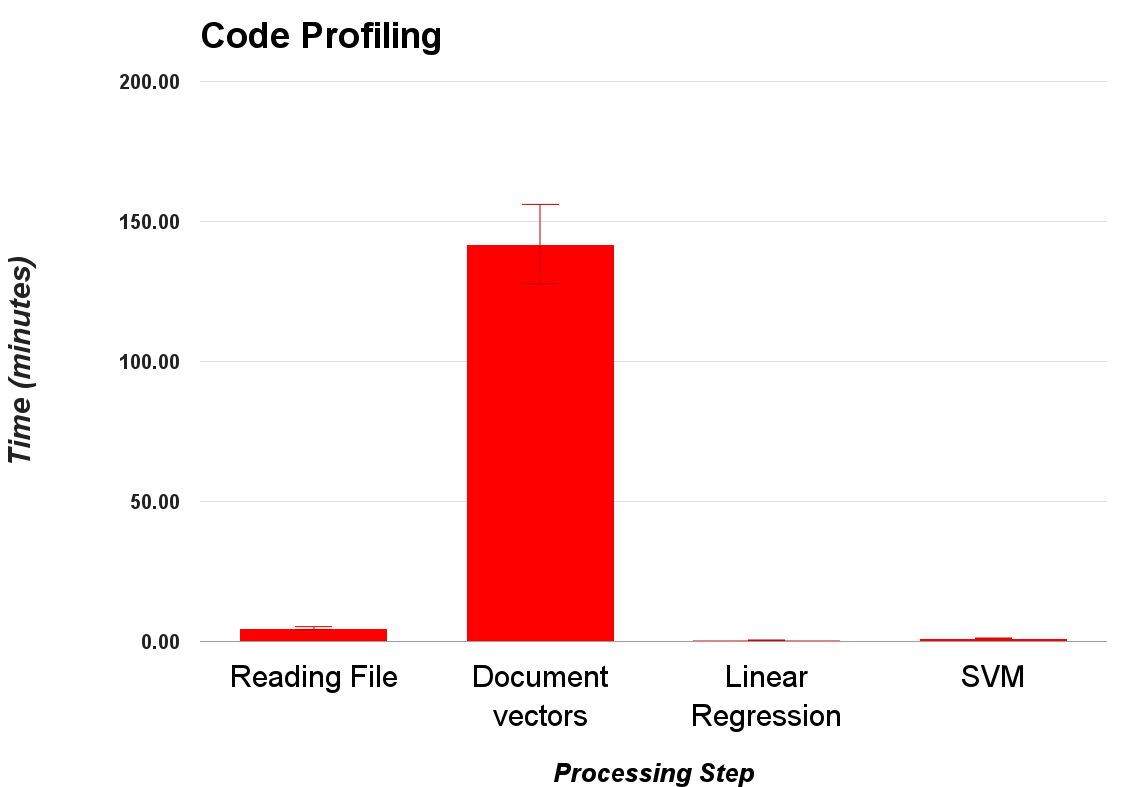
\includegraphics[width=.8\textwidth]{images/code-profiling.png}
\end{frame}

\begin{frame}{Visualization Dashboard}
	\centering
	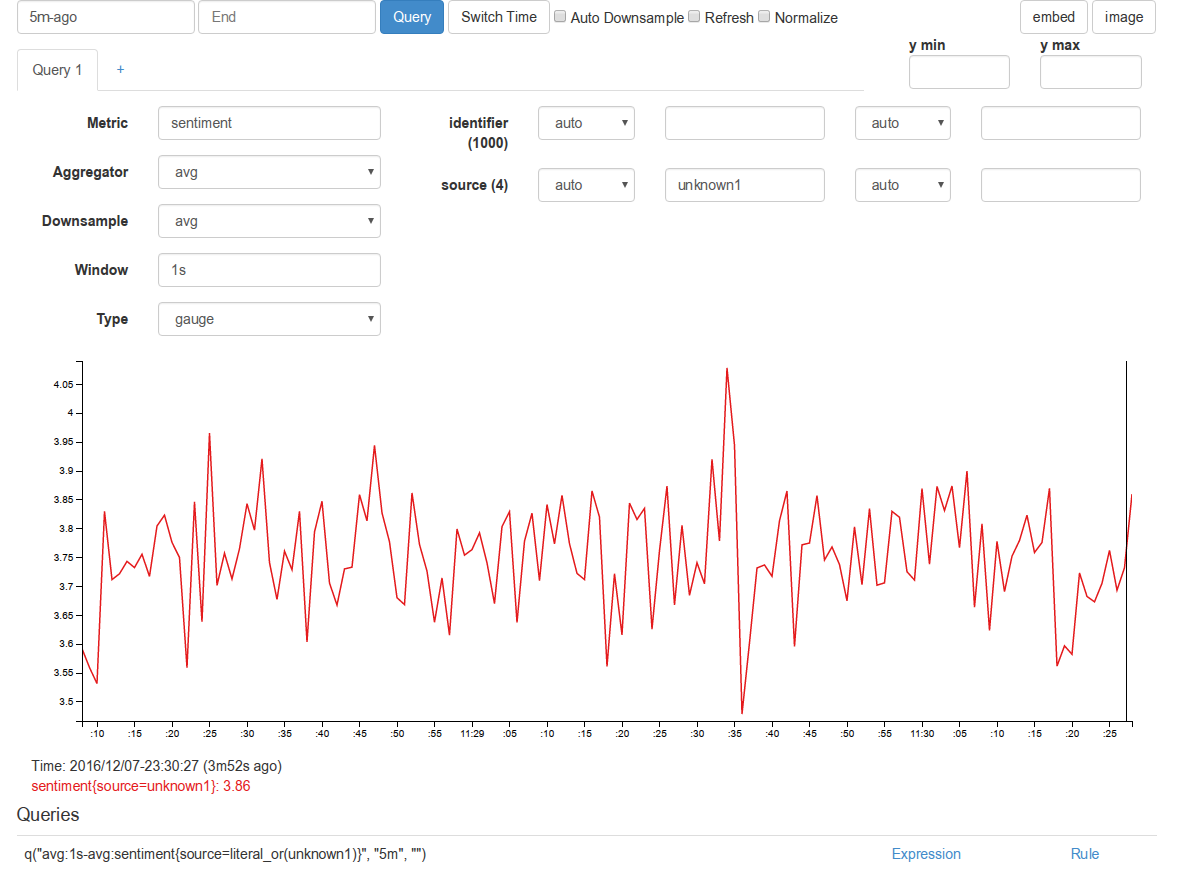
\includegraphics[width=.7\textwidth]{images/bosun-dash.png}
\end{frame}

\begin{frame}{Commentary}
	\begin{columns}[T] % align columns
		\begin{column}{.48\textwidth}
			\color{tropicalrainforest}\rule{\linewidth}{4pt}
			\begin{itemize}
				\item No manual feature engineering or data cleaning needed
				\item Real-time dashboard is as easy to setup as a web-server
				\item Loosely-coupled architecture allows the individual components (Learning Model, Spark Streaming Processor, Time Series viz.) to be used independently of each other.
			\end{itemize}
		\end{column}
		\hfill
		\begin{column}{.48\textwidth}
			\color{usccardinal}\rule{\linewidth}{4pt}
			\begin{itemize}
				\item Quality of the results are low because the paragraph vector model is an oversimplification of how to learn document embeddings.
				\item $R^2$ isn't intuitively helpful in determining how good the model is. RMSE might be a better option.
			\end{itemize}
		\end{column}
	\end{columns}
\end{frame}

\begin{frame}{References}
	\begin{itemize}
		\item Mikolov, Tomas, et al. "Efficient estimation of word representations in vector space." arXiv preprint arXiv:1301.3781 (2013). \footnote{https://www.tensorflow.org/tutorials/word2vec}
		\item Mikolov, Tomas, et al. "Distributed representations of words and phrases and their compositionality." Advances in neural information processing systems. 2013.
		\item Le, Quoc, and Tomas Mikolov. "Distributed representations of sentences and documents." International Conference on Machine Learning. 2014.
	\end{itemize}
\end{frame}

\begin{frame}
	\centering
	\Huge{Questions?}
\end{frame}

\end{document}
